% Formula sheet for MEC E 371 Heat Transfer
% Two column format

\documentclass[9pt]{extarticle}
\usepackage{amsmath}
\usepackage{amssymb}
\usepackage{multicol}
\usepackage{geometry}
\usepackage{fancyhdr}
\usepackage{siunitx}
\usepackage{enumitem}
\usepackage{multicol}
\usepackage{graphicx}
\usepackage{multirow}
\usepackage{lastpage}
\usepackage[final]{hyperref}
\usepackage{parskip}
\usepackage{float}
\usepackage{subcaption}
\usepackage{booktabs}
\usepackage{multirow}
\usepackage{longtable}

%\geometry{letterpaper, portrait, margin=0.5in, footskip=0.25in, top = 0.75in, headsep=0.25in}
\geometry{letterpaper, portrait, margin=0.5in, footskip=0.25in, top = 0.75in, headsep=0.25in}

\setlength{\columnsep}{0.5in}

\hypersetup{
	colorlinks=true,       % false: boxed links; true: colored links
	linkcolor=blue,        % color of internal links
	citecolor=blue,        % color of links to bibliography
	filecolor=magenta,     % color of file links
	urlcolor=blue         
}

\pagestyle{fancy}
\fancyhf{}
\lhead{MEC E 451 Formula Sheet}
\chead{Last Updated: \today}
\rhead{Alex Diep}
\cfoot{\thepage\ of \pageref{LastPage}}

\begin{document}
%\maketitle
%\thispagestyle{empty}
\setlength{\belowdisplayskip}{4pt} \setlength{\belowdisplayshortskip}{0pt}
\setlength{\abovedisplayskip}{4pt} \setlength{\abovedisplayshortskip}{0pt}
\section{System Response for Unforced SDOF Systems}
\begin{table}[h]
    \centering
    \caption{Steady State Solutions for Unforced SDOF Systems}
    \begin{tabular}{lc}
        \toprule
        System & Response \\
        \hline \\[-1ex]
        Undamped Spring Mass & \(\displaystyle \frac{v_0}{p}\sin(pt) + x_0\cos(pt)\) \\[3ex]
        Damped Spring Mass & \(\displaystyle e^{-\zeta pt}\left[\frac{v_0 + \zeta p x_0}{\sqrt{1 - \zeta^2}p}\sin(\sqrt{1 - \zeta^2}p t) + x_0 \cos(\sqrt{1 - \zeta^2} pt)\right]\) \\
        \bottomrule
    \end{tabular}
\end{table} 

\section{Steady State Solutions for Forced SDOF Systems}
\begin{longtable}{lccc}
    \caption{Steady State Solutions for Forced SDOF Systems} \\
        \toprule
        System & Steady State & DMF & Transmissibility \\
        & & (or Amplitude Response) & \\
        \midrule \midrule
        \multicolumn{4}{c}{Undamped Forced Spring Mass} \\
        \midrule 
        Forced Spring Mass & \(\displaystyle \left(\frac{F_0}{k}\right)\left(\frac{1}{1 - \left(\frac{\omega}{p}\right)^2}\right)\sin(\omega t)\) & \(\displaystyle \frac{\mathbb{X}}{\delta_{\text{ST}}} = \frac{1}{\bigg|1-\left(\frac{\omega}{p}\right)^2\bigg|} \) & \(\displaystyle \frac{F_{T_{\text{max}}}}{F_0} = \frac{1}{\bigg|1-\left(\frac{\omega}{p}\right)^2\bigg|}\) \\[6ex]
        Rotating Imbalance & \(\displaystyle \frac{F_0/k}{\big|1-\left(\frac{\omega}{p}\right)^2\bigg|}\sin(\omega t - \phi)\) & \(\displaystyle \frac{M \mathbb{X}}{\tilde{m} e} = \frac{\left(\frac{\omega}{p}\right)^2}{\bigg|1-\left(\frac{\omega}{p}\right)^2\bigg|}\) & \(\displaystyle \frac{F_{T_{\text{max}}}}{\tilde{m}e\omega^2} = \frac{1}{\bigg|1-\left(\frac{\omega}{p}\right)^2\bigg|}\) \\[6ex]
        Base Excitation & \(\displaystyle a \left(\frac{1}{1 - \left(\frac{\omega}{p}\right)^2}\right) \sin(\omega t)\) & \(\displaystyle \frac{\mathbb{X}}{a} = \frac{1}{\bigg|1-\left(\frac{\omega}{p}\right)^2\bigg|}\) & \(\displaystyle \frac{F_{T_{\text{max}}}}{ka} = \frac{\left(\frac{\omega}{p}\right)^2}{\bigg|1-\left(\frac{\omega}{p}\right)^2\bigg|}\) \\
        \midrule 
        \multicolumn{4}{c}{Damped Forced Spring Mass} \\
        \midrule
        % nondimensionalizing the amplitude response
        %Forced Spring Mass & \(\displaystyle \frac{F_0}{\sqrt{(k - m\omega^2)^2 + (c\omega)^2}}\) & \(\displaystyle \frac{\mathbb{X}}{\delta_{\text{ST}}} = \frac{1}{\sqrt{\left[1 - \left(\frac{\omega}{p}\right)^2\right]^2 + \left(2\zeta\frac{\omega}{p}\right)^2}}\) & \(\displaystyle \frac{\sqrt{1 + \left(2 \zeta \frac{\omega}{p}\right)^2}}{\sqrt{\left[1 - \left(\frac{\omega}{p}\right)^2\right]^2 + \left(2\zeta\frac{\omega}{p}\right)^2}}\) \\[6ex]
        Forced Spring Mass & \(\displaystyle \frac{F_0 / k}{\sqrt{\left[1 - \left(\frac{\omega}{p}\right)^2\right]^2 + \left(2\zeta\frac{\omega}{p}\right)^2}}\) & \(\displaystyle \frac{\mathbb{X}}{\delta_{\text{ST}}} = \frac{1}{\sqrt{\left[1 - \left(\frac{\omega}{p}\right)^2\right]^2 + \left(2\zeta\frac{\omega}{p}\right)^2}}\) & \(\displaystyle \frac{F_{T_{\text{max}}}}{F_0} = \frac{\sqrt{1 + \left(2 \zeta \frac{\omega}{p}\right)^2}}{\sqrt{\left[1 - \left(\frac{\omega}{p}\right)^2\right]^2 + \left(2\zeta\frac{\omega}{p}\right)^2}}\) \\[6ex]
        Rotating Imbalance & \(\displaystyle \frac{\tilde{m}e \omega^2 / k}{\sqrt{\left[1 - \left(\frac{\omega}{p}\right)^2\right]^2 + \left(2\zeta\frac{\omega}{p}\right)^2}}\) & \(\displaystyle \frac{M \mathbb{X}}{\tilde{m} e} = \frac{\left(\frac{\omega}{p}\right)^2}{\sqrt{\left[1 - \left(\frac{\omega}{p}\right)^2\right]^2 + \left(2\zeta\frac{\omega}{p}\right)^2}}\) & \(\displaystyle \frac{F_{T_{\text{max}}}}{\tilde{m}e \omega^2} = \frac{\sqrt{1 + \left(2 \zeta \frac{\omega}{p}\right)^2}}{\sqrt{\left[1 - \left(\frac{\omega}{p}\right)^2\right]^2 + \left(2\zeta\frac{\omega}{p}\right)^2}}\) \\[6ex]
        \multirow{2}{*}{Base Excitation} & \(\displaystyle \frac{a \sqrt{k^2 + (c \omega)^2}/k}{\sqrt{\left[1 - \left(\frac{\omega}{p}\right)^2\right]^2 + \left(2\zeta\frac{\omega}{p}\right)^2}}\) & \(\displaystyle \frac{\mathbb{X}}{a} = \frac{\sqrt{1 + \left(2 \zeta \frac{\omega}{p}\right)^2}}{\sqrt{\left[1 - \left(\frac{\omega}{p}\right)^2\right]^2 + \left(2\zeta\frac{\omega}{p}\right)^2}}\) & \(\displaystyle \frac{F_{T_{\text{max}}}}{ka} = \frac{\left(\frac{\omega}{p}\right)^2 \sqrt{1 + \left(2 \zeta \frac{\omega}{p}\right)^2}}{\sqrt{\left[1 - \left(\frac{\omega}{p}\right)^2\right]^2 + \left(2\zeta\frac{\omega}{p}\right)^2}}\) \\
        & &\(\displaystyle \frac{\mathbb{Z}}{a} = \frac{\left(\frac{\omega}{p}\right)^2}{\sqrt{\left[1 - \left(\frac{\omega}{p}\right)^2\right]^2 + \left(2\zeta\frac{\omega}{p}\right)^2}}\) & \\
        \bottomrule
\end{longtable}
General solution for forced damped SDOF system \footnote[1]{$F_0$ for spring, imbalance, and excitation is $F_0$, $m e \omega^2$, and $a\sqrt{k^2+(c\omega)^2}$, respectively.} 
\begin{align*}
    m_{\text{eff}} \ddot{x} + c_{\text{eff}} \dot{x} + k_{\text{eff}} x = F_0 \sin(\omega t - \alpha)
\end{align*}
is given by
\begin{align*}
    x(t) = \mathbb{X} \sin(\omega t - \alpha - \phi)
\end{align*}
where
\begin{align*}
    \mathbb{X} &= \frac{F_0}{\sqrt{\left(k_{\text{eff}} - m_{\text{eff}} \omega^2 \right)^2 + \left(c_{\text{eff}} \omega \right)^2}} = \frac{F_0/k}{\sqrt{\left[1 - \left(\frac{\omega}{p}\right)^2\right]^2 + \left(2\zeta\frac{\omega}{p}\right)^2}} \\
\end{align*}

\section{Steady State Solutions for Forced Non-Harmonic SDOF Systems}
The general steady state solution for a periodic ($\tau = 2\pi/\omega$) forced damped SDOF system is given by:
\begin{align*}
    x(t) = \frac{a_0}{2k} &+ \sum_{j = 1}^{\infty} \frac{a_j/k}{\sqrt{\left[1 - \left(\frac{\omega}{p}\right)^2\right]^2 + \left(2\zeta\frac{\omega}{p}\right)^2}}\cos(j\omega t - \phi_j) \\
    &+ \sum_{j = 1}^{\infty} \frac{b_j/k}{\sqrt{\left[1 - \left(\frac{\omega}{p}\right)^2\right]^2 + \left(2\zeta\frac{\omega}{p}\right)^2}}\sin(j\omega t - \phi_j)
\end{align*}
where
\begin{align*}
    \phi_j &= \tan^{-1} \left[\frac{2\zeta\frac{\omega}{p}}{1 - \left(\frac{j \omega}{p}\right)^2}\right]\\
    a_0 &= \frac{2}{\tau} \int_0^{\tau} F(t) dt = 2 F_{\text{avg}} \\
    a_j &= \frac{2}{\tau} \int_0^{\tau} F(t) \cos(j\omega t) dt, \quad j = 1, 2, 3, \ldots \\
    b_j &= \frac{2}{\tau} \int_0^{\tau} F(t) \sin(j\omega t) dt, \quad j = 1, 2, 3, \ldots
\end{align*}
Todo:
add common solutions such as step, ramp. Ask TA if you can infer some coefficients are zero based on some symmetry.

\section{Transient Response of Spring-Mass Systems}
\begin{table}[H]
    \centering
    \caption{Particular Response of Spring-Mass Systems}
    \begin{tabular}{lll}
        \toprule
        Input & $F_0$ & Particular Response \\
        \midrule
        Step & $F_0 = F_1$ & $\displaystyle x_p(t) = \frac{F_1}{k}$ \\[2ex]
        Ramp & $F_0 = \beta t$ & $\displaystyle x_p(t) = \frac{\beta}{k}t$ \\[2ex]
        Exponential & $F_0 = F_1 e^{-at}$ & $\displaystyle x_p(t) = \frac{F_1}{ma^2 + k} e^{-at}$ \\
        \bottomrule
        \end{tabular}
\end{table}





% \begin{multicols*}{2}
\section*{2. SDOF Systems}
\subsection*{2.1 Undamped SDOF System}
\subsubsection*{2.1.1 Equation of Motion}
\begin{align*}
    m_{\text{eff}} \ddot{x} + k_{\text{eff}}x &= 0 \\
    \ddot{x} + p^2x &= 0
\end{align*}
where $p = \sqrt{\frac{k_{\text{eff}}}{m_{\text{eff}}}}$ is the natural frequency of the system. The general solution to this equation is
\begin{align*}
    x(t) = A\sin(pt) + B\cos(pt)
\end{align*}
If the system is subjected to initial conditions $x(0) = x_0$ and $\dot{x}(0) = v_0$, the solution becomes
\begin{align*}
    x(t) = \left(\frac{v_0}{p}\right)\sin(pt) + x_0\cos(pt)
\end{align*}
the single-term solution is
\begin{align*}
    x(t) = \sqrt{x_0^2 + \left(\frac{v_0}{p}\right)^2}\sin\left(pt + \phi\right) \\
    \phi = \arctan\left(\frac{x_0}{v_0/p}\right)
\end{align*}
and period of oscillation is
\begin{align*}
    \tau = \frac{2\pi}{p}
\end{align*}

\subsubsection{2.1.2 Energy Methods}
When a spring is displaced from its equilibrium position by some $x$, the potential energy stored in the spring is
\begin{align*}
    U = \frac{1}{2}kx^2
\end{align*}
Similarly, the kinetic energy of the mass is
\begin{align*}
    T = \frac{1}{2}m\dot{x}^2
\end{align*}

\subsection{2.2 Spring-Mass Vertical Systems}
All equations hold from the previous section if you consider the spring from its equilibrium position. If the spring is considered at its unstretched length, then $X_0$, the static deflection, is added to the displacement $x$.

\subsection{2.3 Equivalent Mass and Stiffness}
\subsubsection{2.3.1 Equivalent Mass}
Effective mass can be found by finding the total kinetic energy of the system and equating it to the kinetic energy of an effective mass $m_{\text{eff}}$.
\begin{align*}
    T = \frac{1}{2}m_{\text{eff}}\dot{q}^2 = \sum \frac{1}{2}m_i\dot{q}_i^2
\end{align*}
where $q$ is the generalized coordinate.

\subsubsection{2.3.2 Equivalent Stiffness}
Similarly, effective stiffness can be found by equating the total potential energy of the system to the potential energy of an effective spring $k_{\text{eff}}$.
\begin{align*}
    U = \frac{1}{2}k_{\text{eff}}q^2 = \sum \frac{1}{2}k_iq_i^2
\end{align*}
however, stiffness and flexibility approaches are preferred. For the stiffness approach, apply a unit displacement ($\Delta$ or $\theta = 1$) then find the force or moment. For the flexibility approach, apply a unit force or moment ($F = 1$ or $M = 1$) then find the displacement or angle. Assume the system is static. 

For linear and angular displacements respectively,
\begin{align*}
    F &= k_{\text{eff}} \Delta \\
    M &= k_{\text{eff}} \theta
\end{align*}


\end{multicols*}
% \newpage
% \begin{multicols*}{2}
\section*{4. Forced Vibrations of SDOF Systems}
\subsection*{4.1 Simple Spring-Mass Systems}
Consider a simple spring mass system that is forced by $F_0 \sin(\omega t)$ in the direction of motion. The equation of motion is
\begin{align*}
    m\ddot{x} + c\dot{x} + kx = F_0\sin(\omega t)
\end{align*}
The solution is 
\begin{align*}
    x(t) = x_{H}(t) + x_{P}(t)
\end{align*}
Recall from Section 2.1.1 that the homogeneous solution is
\begin{align*}
    x_H(t) = A\sin(pt) + B\cos(pt)
\end{align*}
The particular solution can be found using the method of undetermined coefficients by assuming $x_P(t) = C\sin(\omega t) + D\cos(\omega t)$. The particular solution is
\begin{align*}
    x_P(t) = \frac{F_0}{k - m\omega^2}\sin(\omega t)
\end{align*}
So, the total response is
\begin{align*}
    x(t) = A\sin(pt) + B\cos(pt) + \frac{F_0}{k - m\omega^2}\sin(\omega t)
\end{align*}
Since most real systems have damping to some degree, we consider only the forced response, which comes from the particular solution. So let the steady state solution be
\begin{align*}
    x(t) &= \frac{F_0}{k - m\omega^2}\sin(\omega t) \\
    &= \frac{F_0}{k} \frac{1}{1 - \left(\frac{\omega}{p}\right)^2}\sin(\omega t) \\
    &= X \sin(\omega t)
\end{align*}
Defining static deflection as 
\begin{align*}
    X_0 = \frac{F_0}{k} \frac{1}{1 - \left(\frac{\omega}{p}\right)^2}
\end{align*}
then, the dynamic magnification factor is
\begin{align*}
    \text{DMF} = \frac{X}{X_0} = \frac{1}{\sqrt{1 - \left(\frac{\omega}{p}\right)^2}}
\end{align*}

\subsubsection*{4.1.1 Resonance Response}
A different form for the particular solution is used when the system is at resonance. By assuming the form $x_P(t) = C t \sin(\omega t) + D t \cos(\omega t)$, the particular solution is
\begin{align*}
    x_P(t) = - \frac{F_0 t}{2mp} \sin(\omega t)
\end{align*}


\end{multicols*}


% \newpage
% \begin{multicols*}{2}
\section*{11. Heat Exchangers}
\subsection*{11.1. General Procedure}
\subsubsection*{11.1.1. Log Mean Temperature Difference Method}
\begin{enumerate}
    \item See if $\dot{Q}$ is given or can be obtained by energy balance
    \[ \dot{Q} = \dot{m} c_p (T_{\text{out},h} - T_{\text{in},h}) = \dot{m} c_p (T_{\text{in},c} - T_{\text{out},c}) \]
    \item Find the log mean temperature difference, $\Delta T_{\text{lm}}$
    \item Find the heat transfer coefficient, $U$. For multipass shell-and-tube heat exchangers, use
    $A_s = N A_{s,i}$ where $N$ is the number of passes and $A_{s,i}$ is the surface area of one pass.
\end{enumerate}
\subsubsection*{11.1.2. $\varepsilon$-NTU Method}
\begin{enumerate}
    \item Find NTU using the given heat exchanger type and $c$
    \item Find $\varepsilon$ using the given heat exchanger type and NTU
    \item Find $\dot{Q}$ using $\varepsilon$ and $\dot{Q}_{\text{max}}$
    \item 
\end{enumerate}
% Add this to a glossary section later
\subsection*{11.2. Variable Definitions}
\begin{itemize}
    \item $\dot{Q}$: Heat transfer rate
    \item $\dot{Q}_{\text{max}}$: Maximum heat transfer rate
    \item $T_{\text{in},h}$: Hot inlet temperature
    \item $T_{\text{out},h}$: Hot outlet temperature
    \item $T_{\text{in},c}$: Cold inlet temperature
    \item $T_{\text{out},c}$: Cold outlet temperature
    \item $U$: Overall heat transfer coefficient
    \item $\Delta T_{\text{lm}}$: Log mean temperature difference
    \item $F$: Correction factor 
    \item $\varepsilon$: Effectiveness
    \item $\dot{Q}_{\text{max}}$: Maximum heat transfer rate
    \item $C_c$: Cold heat capacity rate
    \item $C_h$: Hot heat capacity rate
    \item $C$: Heat capacity rate ratio
    \item $\text{NTU}$: Number of transfer units
\end{itemize}

\subsection*{11.3. Formulas}
\subsection*{11.3.1. Log Mean Temperature Difference Method}
For a heat exchanger,
\begin{align*}
    \dot{Q} &= \dot{Q}_{c} = -\dot{Q}_{h} 
\end{align*}
Overall heat transfer coefficient,
\begin{align*}
    \frac{1}{U A_s} &= \frac{1}{U_i A_{s,i}} = \frac{1}{U_o A_{s,o}} = R = \frac{1}{h_i A_{s,i}} +
    R_{\text{wall}} + \frac{1}{h_o A_{s,o}} 
\end{align*}
Log mean temperature difference,
\begin{align*}
    \Delta T_{\text{lm}} &= \frac{\Delta T_1 - \Delta T_2}{\ln(\Delta T_1 / \Delta T_2)} \\
    \Delta T_1 &= T_{\text{in},h} - T_{\text{out},c} \\
    \Delta T_2 &= T_{\text{out},h} - T_{\text{in},c} \\
    \dot{Q} &= U A_s \Delta T_{\text{lm}} 
\end{align*}
Correction factor,
\begin{align*}
    \Delta T_{\text{lm}} &= F \Delta T_{\text{lm, CF}} 
\end{align*}
where $\Delta T_{\text{lm, CF}}$ is the log mean temperature difference for counterflow and $F$ is the correction factor
which can be found in Figure \ref{fig:sec11_correction_factor}.

\subsection*{11.3.2. $\varepsilon$-NTU Method}
\begin{align*} 
    C_{\text{min}} &= \min(\dot{m}_c c_{p,c}, \dot{m}_h c_{p,h}) \\
    \dot{Q}_{\text{max}} &= C_{\text{min}} (T_{\text{in},h} - T_{\text{in},c}) \\
    \dot{Q} &= C_c (T_{\text{out},c} - T_{\text{in},c}) = C_h (T_{\text{in},h} - T_{\text{out},h}) \\
    \epsilon &= \frac{\dot{Q}}{\dot{Q}_{\text{max}}} \\
\end{align*}
if $C_c = C_{\text{min}}$,
\begin{align*}
    \epsilon &= \frac{\dot{Q}}{\dot{Q}_{\text{max}}} = \frac{T_{\text{out}, c} - T_{\text{in}, c}}{T_{\text{in}, h} - T_{\text{in}, c}} 
\end{align*}
if $C_h = C_{\text{min}}$,
\begin{align*}
    \epsilon &= \frac{\dot{Q}}{\dot{Q}_{\text{max}}} = \frac{T_{\text{in}, h} - T_{\text{out}, h}}{T_{\text{in}, h} - T_{\text{in}, c}}
\end{align*}
NTU is defined as,
\begin{align*}
    \text{NTU} &= \frac{UA_{s}}{C_{\text{min}}} = \frac{UA_{s}}{\dot{m} c_{p, \text{min}}} \\
    c &= \frac{C_{\text{min}}}{C_{\text{max}}} 
\end{align*}
The effectiveness, $\varepsilon$, can be found using Table \ref{tab:sec11_effectiveness_relations}.



\end{multicols*}
    
\section*{Tables}
\begin{figure}[H]
    \centering
    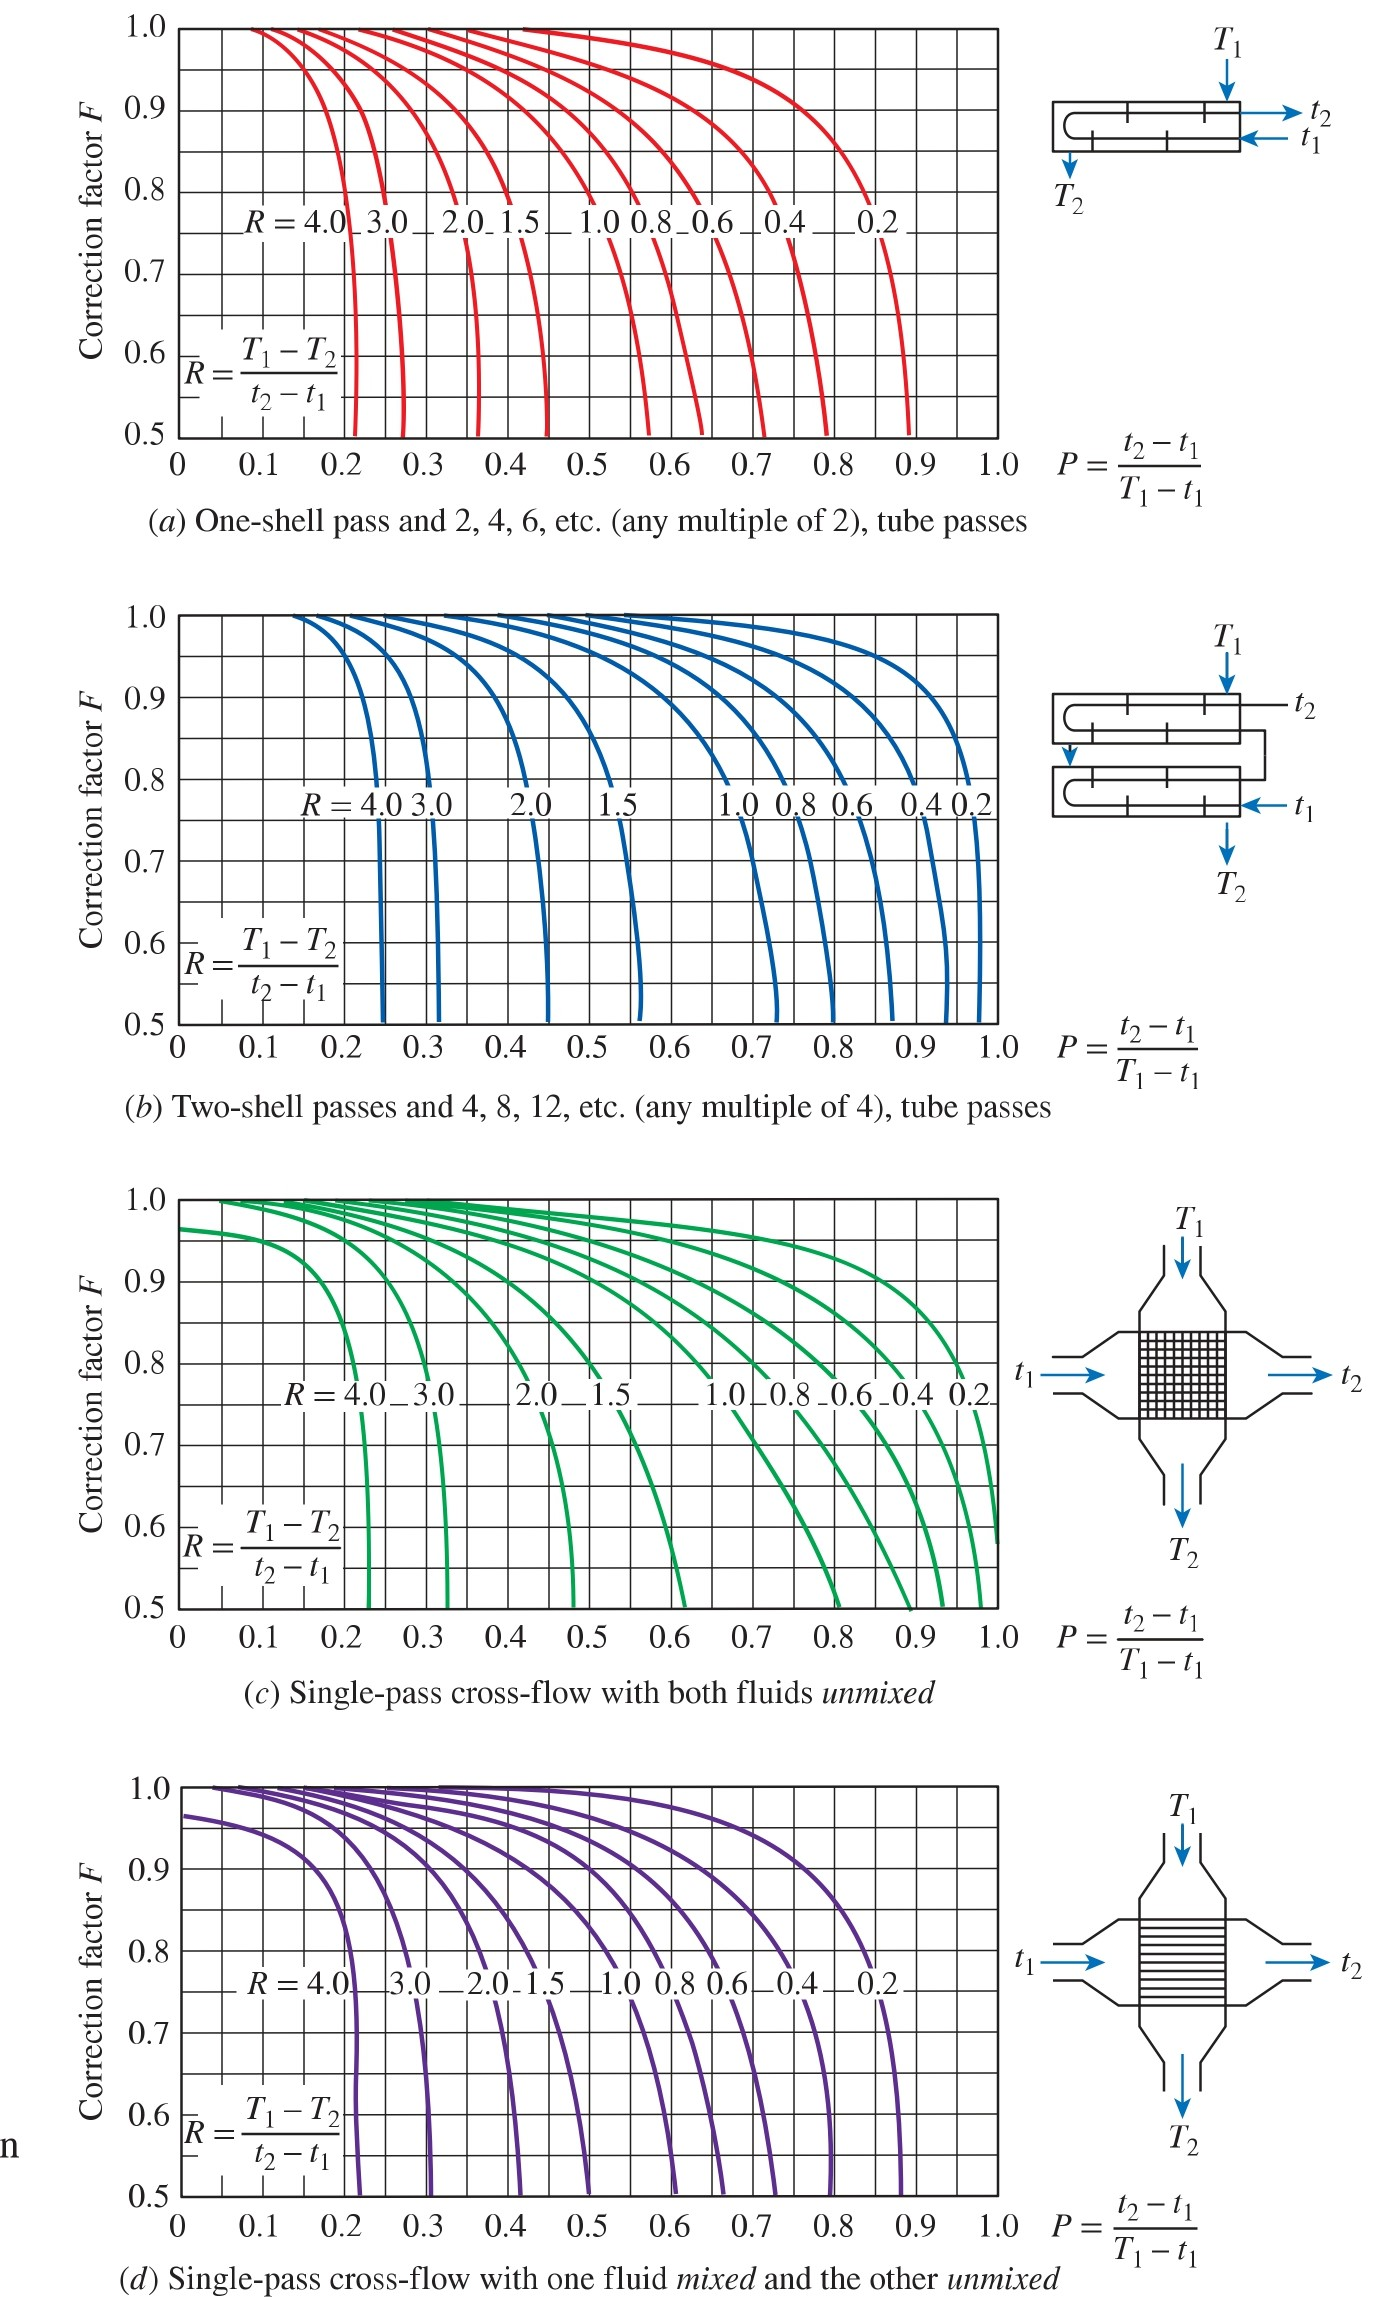
\includegraphics[width=0.7\linewidth]{Figures/Sec11 11-9.jpg}
    \caption{Correction factor F charts for common 
    shell-and-tube and crossflow heat 
    exchangers.}
    \label{fig:sec11_correction_factor}
\end{figure}
\newpage
\begin{table}[H]
    \centering
    \caption{Effectiveness relations for heat exchangers: NTU = $UA_s/C_{\text{min}}$ and $c = C_{\text{min}}/C_{\text{max}} =
    (\dot{m} c_p)_{\text{min}}/(\dot{m} c_p)_{\text{max}}$}
    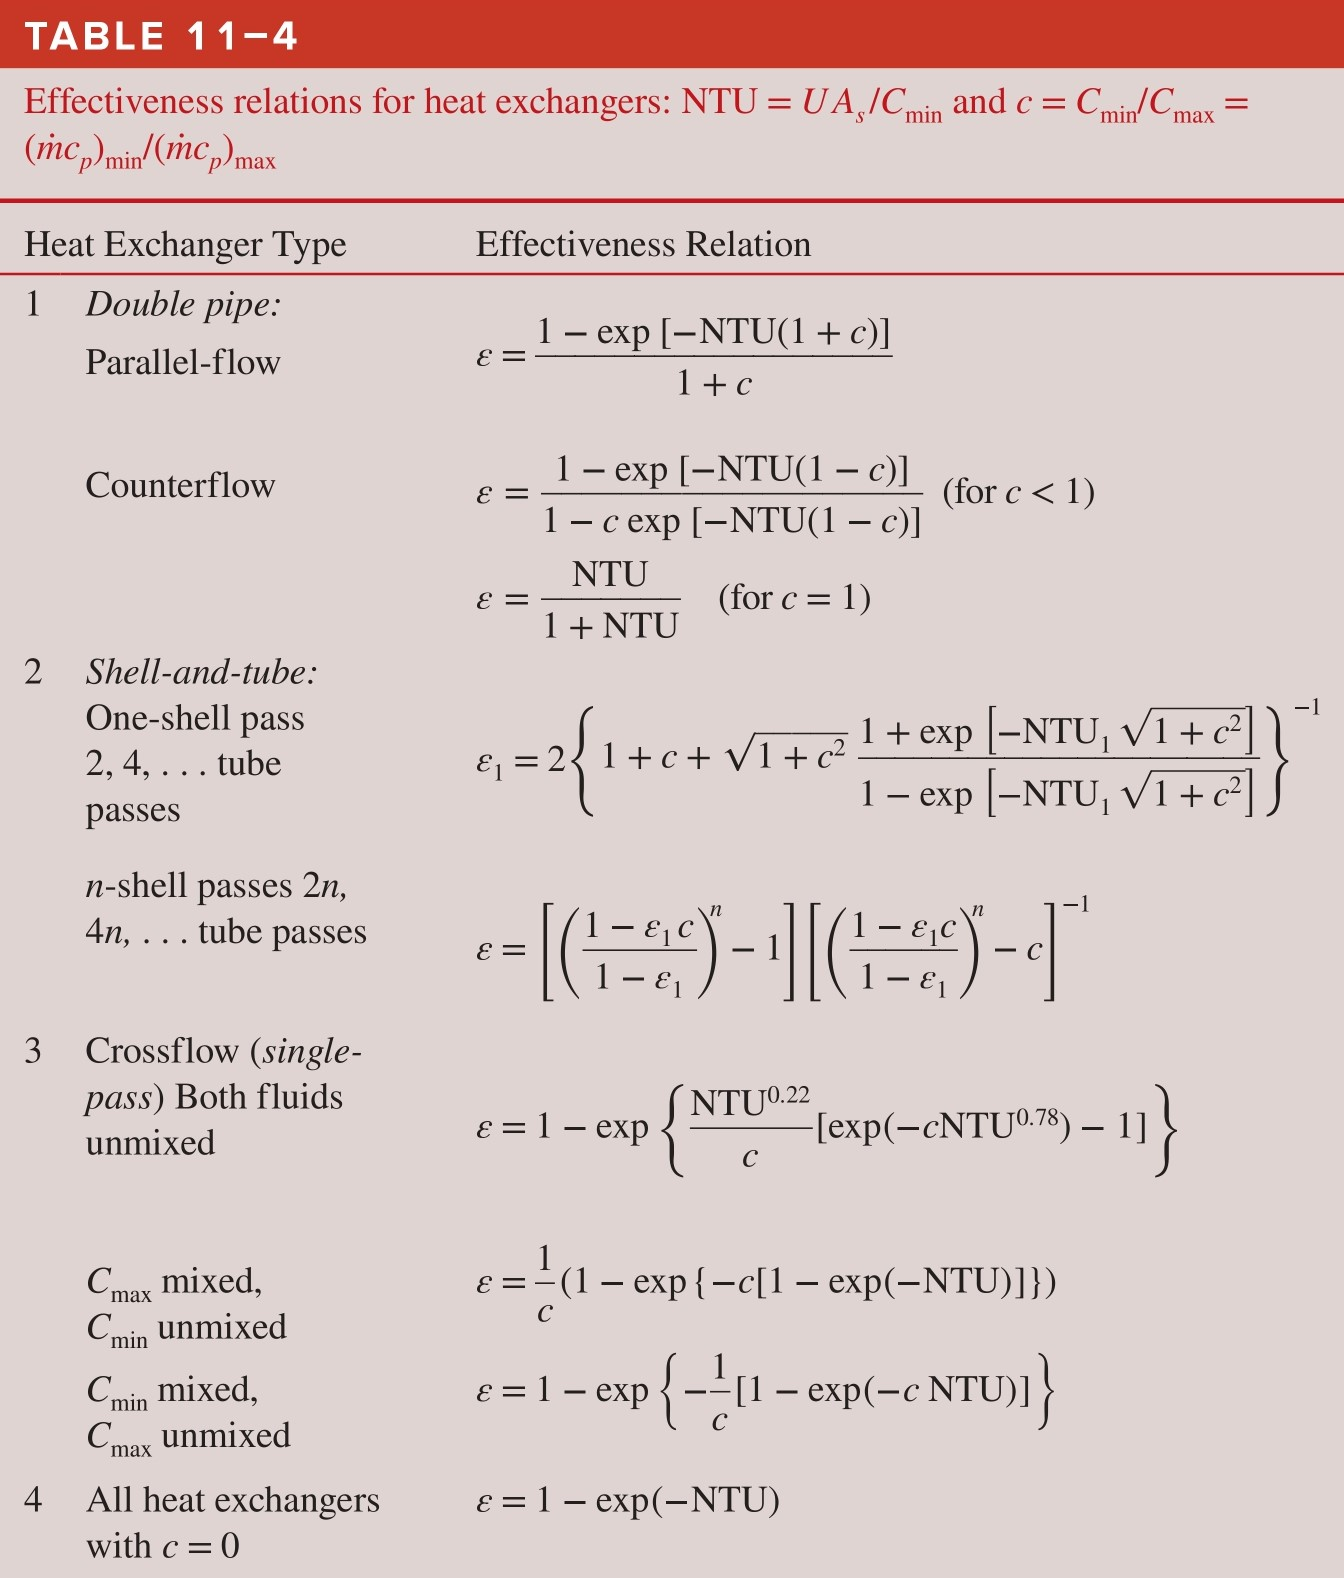
\includegraphics[width=0.8\linewidth]{Figures/Sec11 table 11-4.jpg}
    \label{tab:sec11_effectiveness_relations}
\end{table}
    
% \newpage
% \begin{multicols*}{2}
\section*{12. Thermal Radiation Fundamentals}
\subsection*{12.1. General Procedure}
Most questions will ask for irradiation given some geometry and temperatures.
\begin{enumerate}
    \item Determine absorptivity $\alpha$, reflectivity $\rho$, and transmissivity $\tau$ using the geometry and material properties. 
    Note that if two of these are known, the third can be found using $\alpha + \rho + \tau = 1$.
    \item Use solid angle $\omega$, irradiation $G$, and intensity $I$ to find whatever is asked for
\end{enumerate}
\subsection*{12.2. Variable Definitions}
\begin{itemize}
    \item $\omega$: Solid angle
    \item $G$: Irradiation
    \item $I$: Intensity
    \item $J$: Radiosity
    \item $\dot{Q}$: Heat transfer rate
    \item $\alpha$: Absorptivity
    \item $\rho$: Reflectivity
    \item $\tau$: Transmissivity
    \item $\epsilon$: Emissivity
    \item $\sigma$: Stefan-Boltzmann constant
\end{itemize}

\subsection*{12.3. Formulas}
For $A \ll r^2$ (small area, far away from surface),
\begin{align*}
    \omega_{2-1} &:= \frac{A_2 \cos\theta_2}{r^2}\\
    J_1 &:= \pi I_{1, e+r} = E_b + G_{\text{ref}} = \epsilon\sigma T_{1}^4  + \rho G_{1} \\ 
    \dot{Q}_{1-2} &:= I_1 (A_1 \cos\theta_1) \omega_{2-1} \\
    G_2 &:= \frac{\dot{Q}_{1-2}}{A_2} 
\end{align*}
Combining the above equations into $G_2$,
\begin{align*}
    G_2 &= \frac{(\epsilon\sigma T_{1}^4  + \rho G_{\text{1}})A_1 \cos\theta_1 \cos\theta_2}{\pi r^2} 
\end{align*}
For $\theta_1 = \theta_2 = \rho = 0$ and $\epsilon = 1$ for a blackbody,
\begin{align*}
    G_2 &= \frac{\sigma T_{1}^4 A_1}{\pi r^2} \\
    \implies T_{1} &= \left(\frac{G_2 \pi r^2}{\sigma A_1}\right)^{1/4}
\end{align*}

\end{multicols*}
% \newpage
% \begin{multicols*}{2}
\section*{13. Thermal Radiation Heat Transfer}
\subsection*{13.1. General Procedure}
Most questions will ask for irradiation given some geometry and temperatures.
\begin{enumerate}
    \item Determine view factors $F_{ij}$ from inspection using the geometry.  Check for special cases such as:
    \begin{itemize}
        \item $F_{ii} = 0$ when the surface $i$ is planar or convex
        \item $F_{ij} = 1$ when the surface $i$ is a concave and fully encloses surface $j$
    \end{itemize}
    \item Check Figures section for view factors that cannot be obtained from inspection
    \item Use the reciprocity relation and summation rule to find the remaining view factors
\end{enumerate}
Solvability condition: Given $N$ surfaces, there are $N^2$ view factors. $N(N-1)/2$ view factors must be 
given by inspection, problem statement, or tables. The rest can be determined using reciprocity and summation.
\subsection*{13.2. Variable Definitions}
\begin{itemize}
    \item $F_{ij}$: View factor, the fraction of radiation leaving surface $i$ that strikes surface $j$ 
    \item $\omega$: Solid angle
    \item $G$: Irradiation, the rate of radiant energy incident on a surface per unit area
    \item $I$: Intensity
    \item $J$: Radiosity, the total rate of radiant energy leaving a surface per unit area
    \item $E_{b}$: Black body emissive power
    \item $\dot{Q}$: Heat transfer rate
    \item $\alpha$: Absorptivity
    \item $\rho$: Reflectivity
    \item $\tau$: Transmissivity
    \item $\epsilon$: Emissivity
    \item $\sigma$: Stefan-Boltzmann constant
\end{itemize}
\subsection*{13.3. Formulas}
Reciprocity relation:
\begin{align*}
    A_{1, s} F_{12} &= A_{2, s} F_{21} 
\end{align*}
Summation rule:
\begin{align*}
    \sum_{j=1}^n F_{ij} &= 1 
\end{align*}
Crossed-strings method:
\begin{figure}[H]
    \centering
    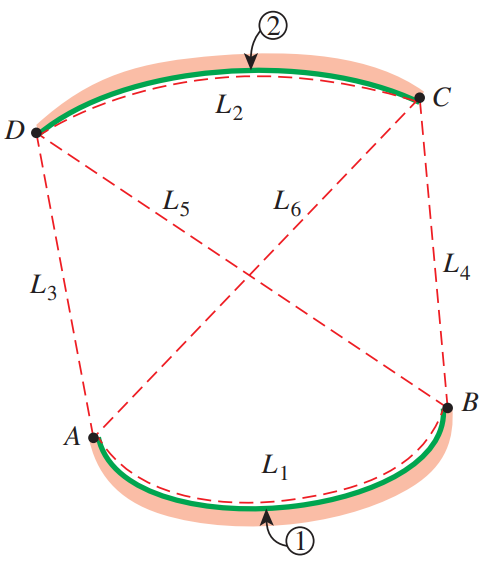
\includegraphics[width=0.2\textwidth]{Figures/Sec13 crossed strings.png}
    \caption{Determination of the view factor $F_{12}$ by the application of the crossed-strings method.}
    \label{fig:sec13_crossed_strings}
\end{figure}
\begin{align*}
    F_{12} &= \frac{(L_5 + L_6) - (L_3 + L_4)}{2 L_1} 
\end{align*}
On a black body, net radiation heat transfer is
\begin{align*}
    E_{bi} &= \sigma T_i^4 \\
    \dot{Q}_{12} &= A_{1, s} F_{12} \sigma (T_1^4 - T_2^4) = A_{2, s} F_{21} \sigma (T_1^4 - T_2^4) 
\end{align*}
On a grey body ($\epsilon_i = \alpha_i$, $\tau = 0$, $\alpha_i + \rho_i =1$), net radiation heat transfer is
\begin{align*}
    J_i &= \pi I_i = \epsilon_i \sigma T_i^4 + \rho_i G_i \\
    \dot{Q}_{12} &= \frac{A_{i, s} \epsilon_{i}}{1 - \epsilon_i} (E_{bi} - J_i) 
\end{align*}
For radiation in two-surface enclosures, net radiation heat transfer is
\begin{align*}
    \dot{Q}_{12} &= \dot{Q}_{1} = -\dot{Q}_{2} \\
    \dot{Q}_{12} &= \frac{\sigma (T_{1}^4 - T_{2}^4)}{\frac{1- \epsilon_1}{\epsilon_1 A_{1, s}} + \frac{1}{A_{2, s} F_{12}} + \frac{1-\epsilon_2}{\epsilon_2 A_{2, s}}} \\
    &= \frac{E_{b1} - E_{b2}}{R_{1} + R_{12} + R_{2}} 
\end{align*}
For some familiar geometries, the above equation simplifies, which is given in Table \ref{tab:sec13_radiation_enclosure_relations}.
\end{multicols*}

\section*{Figures}
\label{sec:sec13_figures}
\begin{figure}[H]
    \centering
    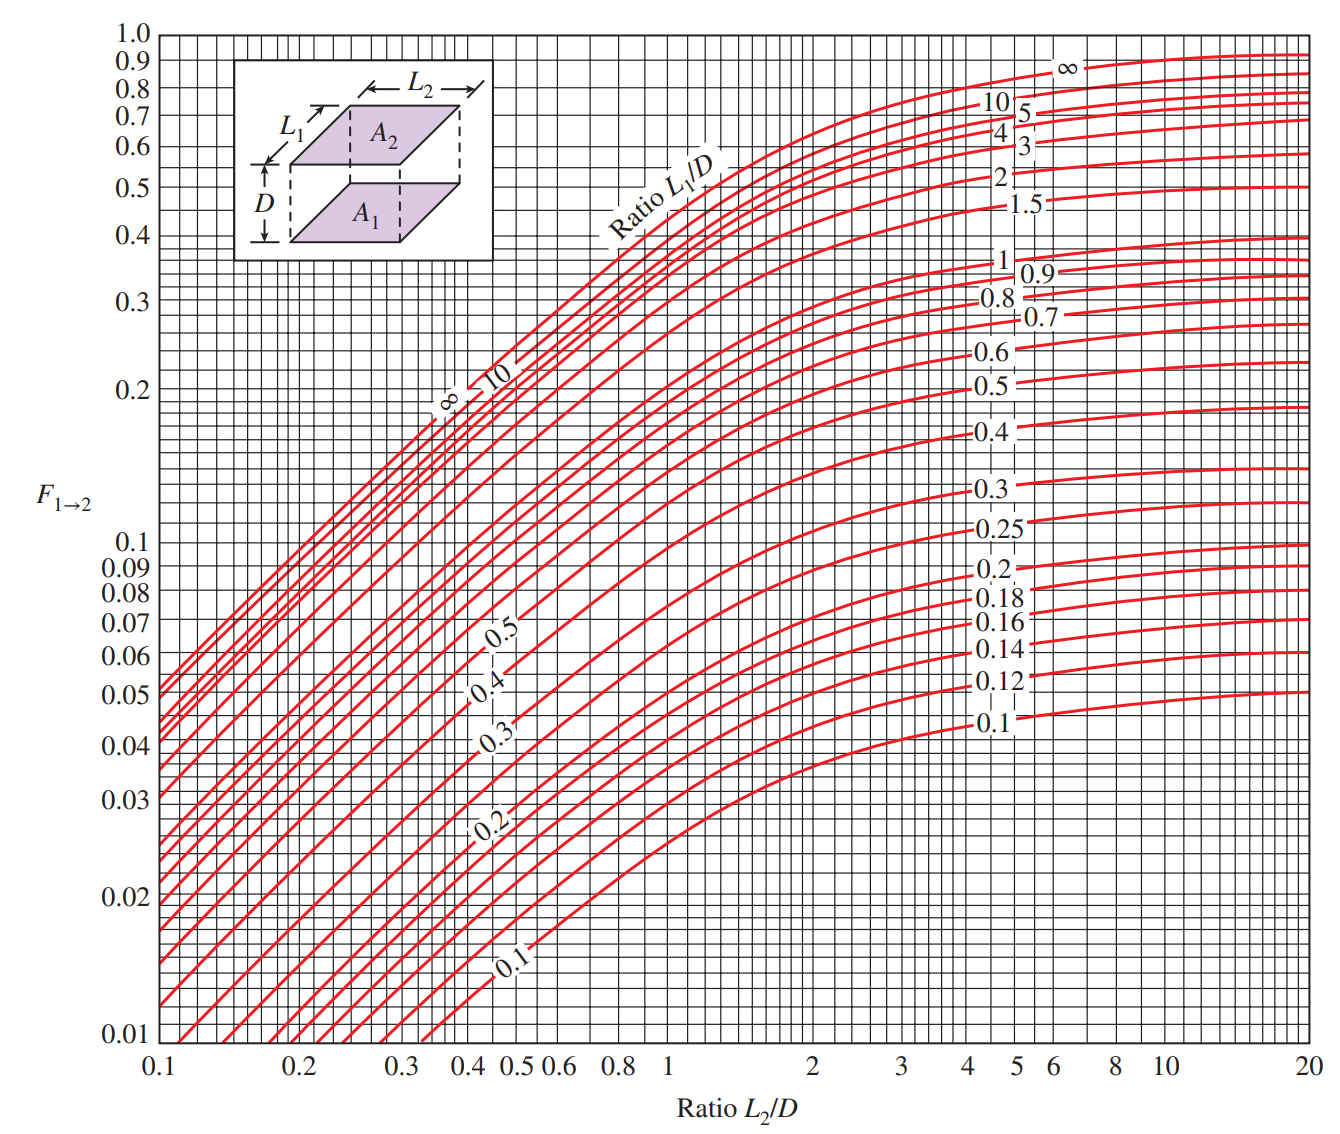
\includegraphics[width=0.6\textwidth]{Figures/Sec13 aligned parallel plates.png}
    \caption{View factor between two aligned parallel rectangles of equal size}
    \label{fig:sec13_aligned_parallel_rectangles}
\end{figure}
\begin{figure}[H]
    \centering
    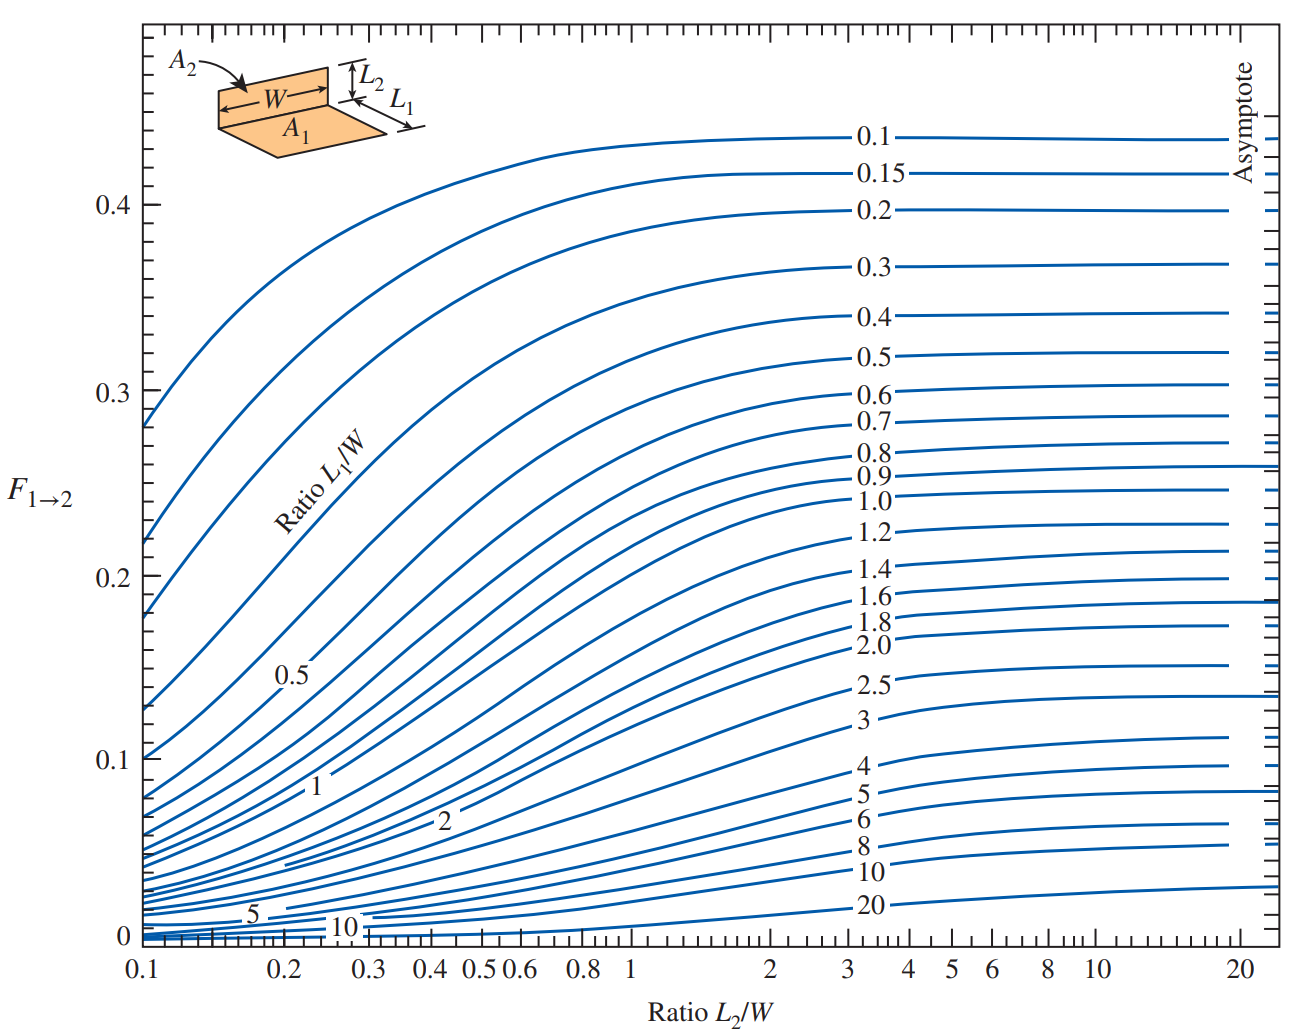
\includegraphics[width=0.6\textwidth]{Figures/Sec13 perpendicular rectangle.png}
    \caption{View factor between two perpendicular rectangles with a common edge}
    \label{fig:sec13_perpendicular_rectangles}
\end{figure}
\begin{figure}[H]
    \centering
    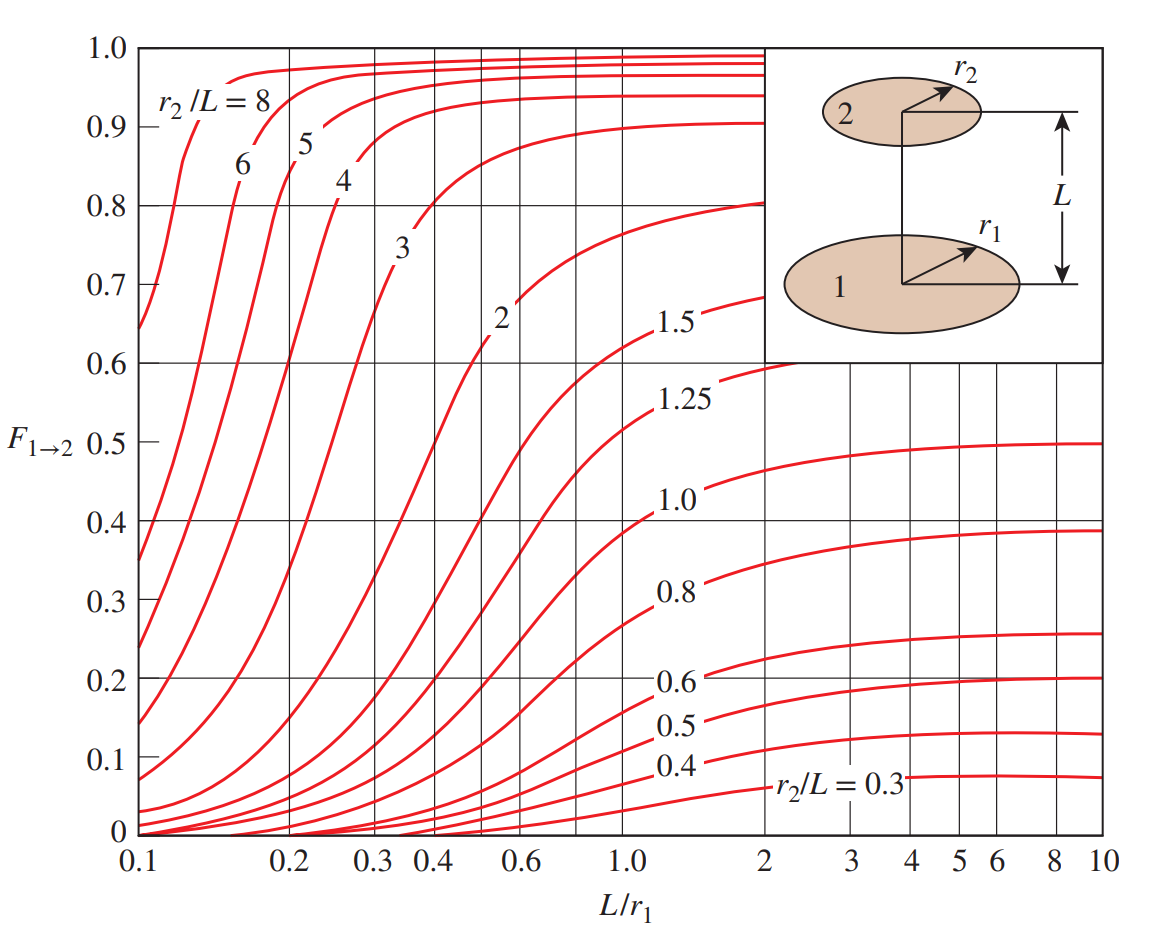
\includegraphics[width=0.6\textwidth]{Figures/Sec13 coaxial parallel disk.png}
    \caption{View factor between two coaxial parallel disks}
    \label{fig:sec13_coaxial_parallel_disks}
\end{figure}
\begin{figure}[H]
    \centering
    \begin{subfigure}[b]{0.4\textwidth}
        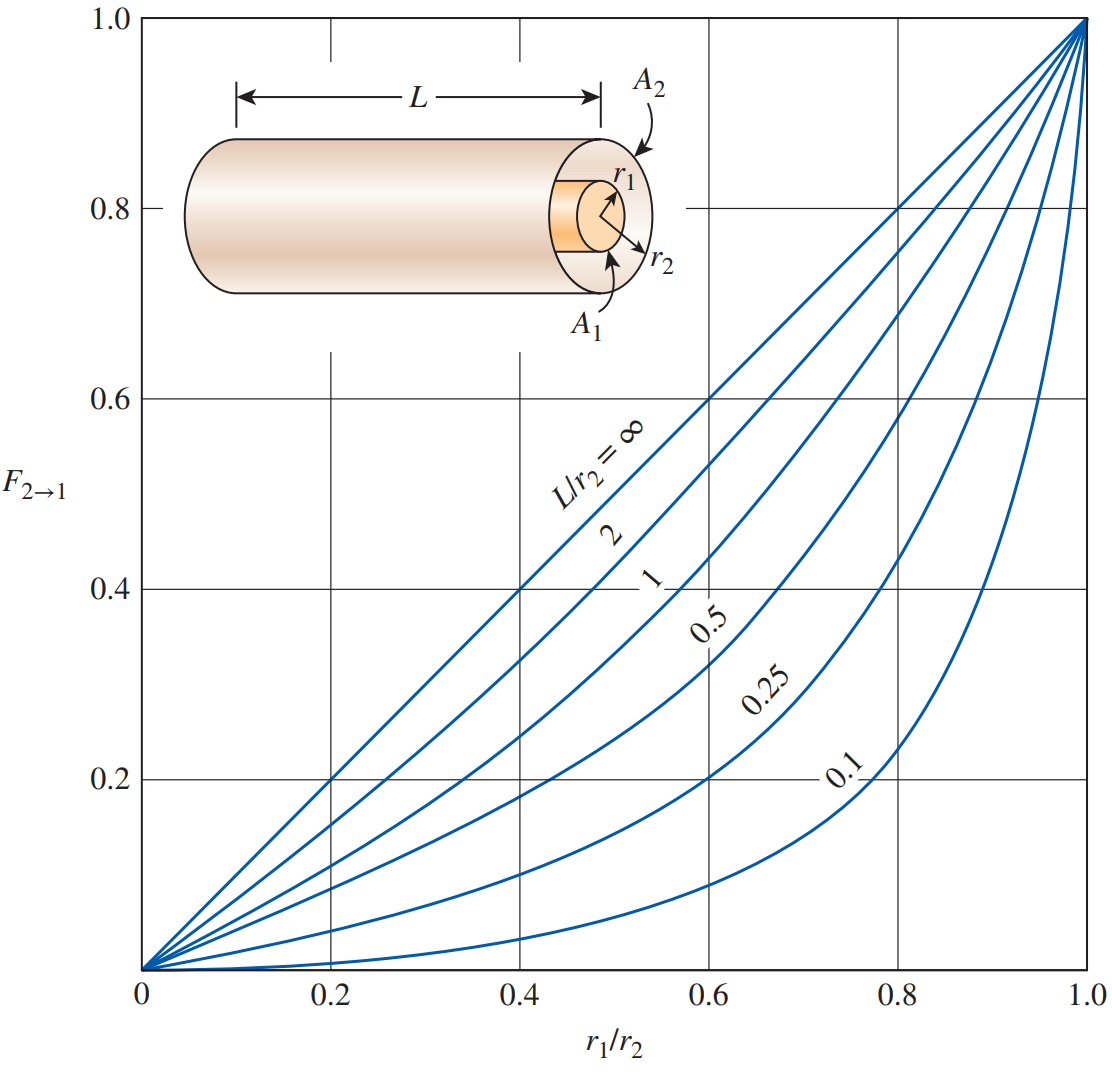
\includegraphics[width=\textwidth]{Figures/Sec13 concentric 2-1.png}
    \end{subfigure}
    \begin{subfigure}[b]{0.4\textwidth}
        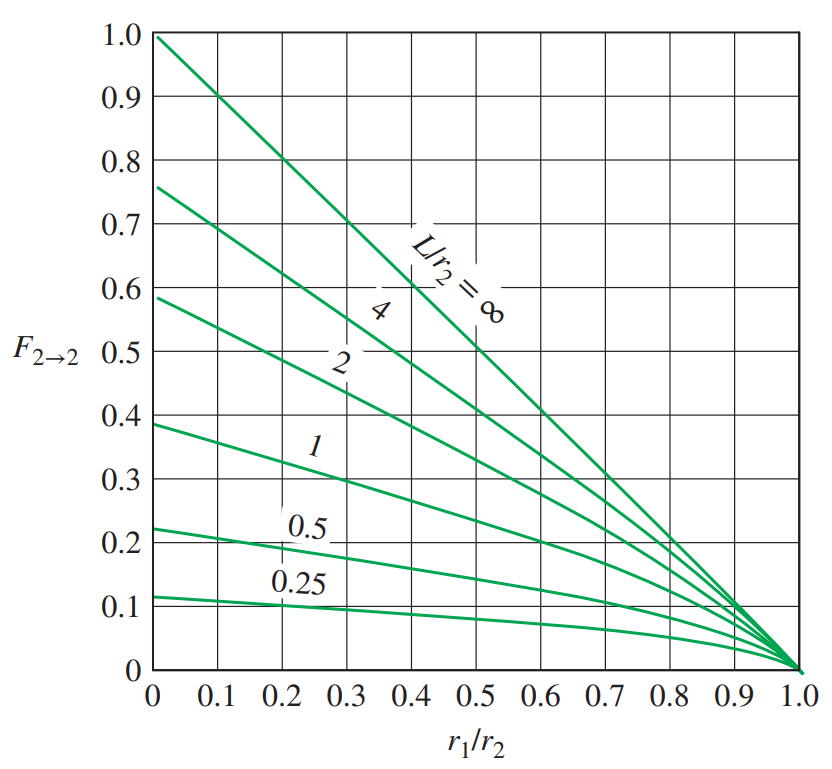
\includegraphics[width=\textwidth]{Figures/Sec13 concentric 2-2.png}
    \end{subfigure}
    \caption{View factors for two concentric cylinders of finite length: (a) outer cylinder to inner cylinder; (b) outer cylinder to itself.}
    \label{fig:sec13_concentric_cylinders}
\end{figure}

\section*{Tables}
\begin{table}[H]
    \centering
    \caption{Radiation heat transfer relations for some familiar two-surface arrangements}
    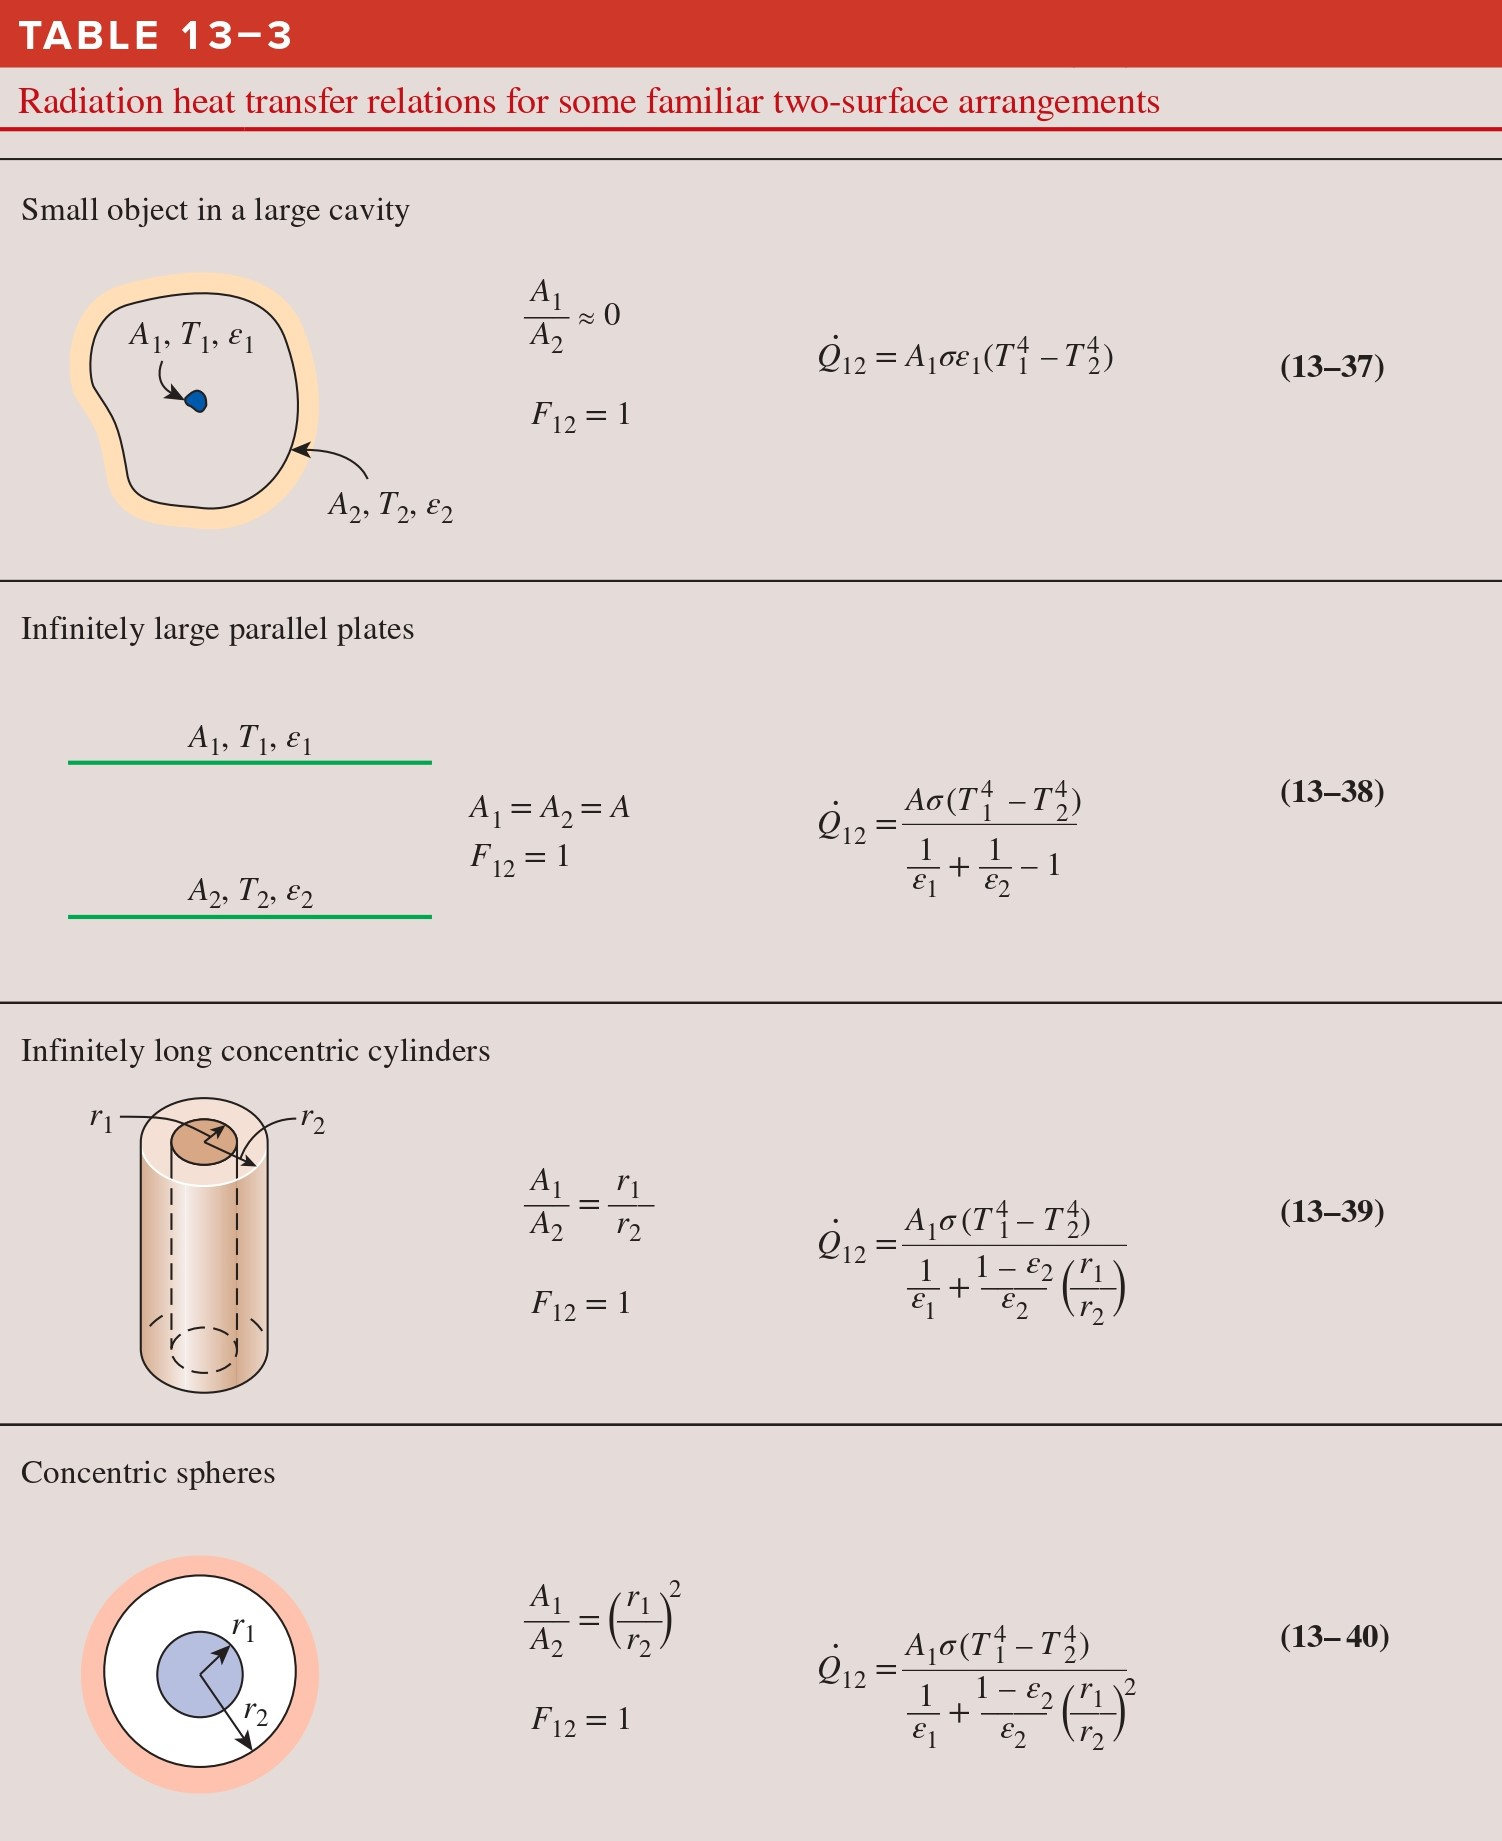
\includegraphics[width=0.8\textwidth]{Figures/Sec13 heat transfer enclosed.png}
    \label{tab:sec13_radiation_enclosure_relations}
\end{table}

\end{document}
